\documentclass[journal=tches,final]{iacrtrans}
%%%% NOTES:
% - Change "journal=tosc" to "journal=tches" if needed
% - Change "submission" to "final" for final version

\usepackage{subcaption}
\usepackage{amsmath}

\author{Paul Cordellier}
\institute{
  Hochschule Albstadt-Sigmaringen, Albstadt-Ebingen, Germany, \email{cordellierp@gmail.com}
}

\title{TLS and SSH Downgrade Attacks and Protections}
%%%% NOTES:
% - If the title is too long, or includes special macro, please
%   provide a "running title" as optional argument: \title[Short]{Long}
% - You can provide an optional subtitle with \subtitle.

\begin{document}

\maketitle

\keywords{Downgrade attack \and OpenSSH \and TLS \and SSL \and Man-in-the-middle}


\begin{abstract}
  As cryptographic systems grow older, vulnerabilities are found in older systems. Unfortunately, some servers or clients aren't updated accordingly. SSL 2.0, a version of TLS' predecessor, is considered deprecated and unsafe since 2011. In 2020, 1.2 million web servers supported this version, and that number decreased to 450 thousand in 2023. \cite{ssl_stats} So we can infer that the unsafe version SSL 3.0 is still widely used.
  
  For communication software developers, this means that making backwards compatible software is important, so that the user can still access websites that are less maintained. Therefore, a system must be implemented so that both client and server understand the secure tools they can use for the communication to be as safe as possible. In a downgrade attack, this system is exploited so that a more vulnerable mode of operation is used. 
  
  This paper will present downgrade attacks present in OpenSSH version 9.4p1 and 9.5p1, and in older TLS version, that enable the attacker to downgrade the communication. This paper also informs of what the industry came up with to fix those issues. 
\end{abstract}


\section{Introduction}

The handshake is a procedure in which two devices or programs attempt to initiate communication and establish their communication parameters. In the following attacks, the client and the server agree on encryption and authentication procedures during the handshake. The attacker plays the role of the man-in-the-middle, altering data during the handshake process.


\section{Man-in-the-middle}
\label{sec:MitM}

At its core, the man-in-the-middle secretly relays the communications, and alters them. In the context of our attacks, the goal is to convince the server that the man-in-the-middle is the client, and vice versa. So the attacker doesn't get spotted, most of the packets are sent back to their intended devices. Here are examples of man-in-the-middle attacks:
 
\begin{itemize}

  \item \textbf{ARP Spoofing}: the ARP (Address Resolution Protocol) links the MAC address and the IP address of the device. The scope of this attack is on a local network. The attacker sends lot of fake ARP information, to convince the victims that the data should be sent to them. This is how the man-in-the-middle fakes its identity. \cite{MitM} Ethernet is a protocol that was designed without any authentication technology. For example, LAN is based on this protocol, so it is relatively easy to perform this attack on this kind of network. \cite{ARP_cache_poisoning}
  
  \item \textbf{DNS Spoofing}: The attacker exploits a vulnerability in a DNS server and injects fake DNS entries. If it works, the domain name will redirect to the attacker's device. This attack often has a larger scale and is harder to perform. \cite{MitM}
 
  \item \textbf{Evil twin attack}: The attacker creates a fake Wi-Fi access point, hoping that victims will connect to it. The attacker should be able to read the data of this fake access point and send any requests they want. This attack can be set up in places with public Wi-Fi, like airports or coffee shops. \cite{evil_twin_attack}
  
  \item \textbf{Man in the Browser}: The victim's browser is exploited, and the attacker can take the position of a man-in-the-middle. This can be set up through a malware or unsafe browser extensions. \cite{man_in_the_browser}
  
\end{itemize}


\begin{figure}
    \centering
    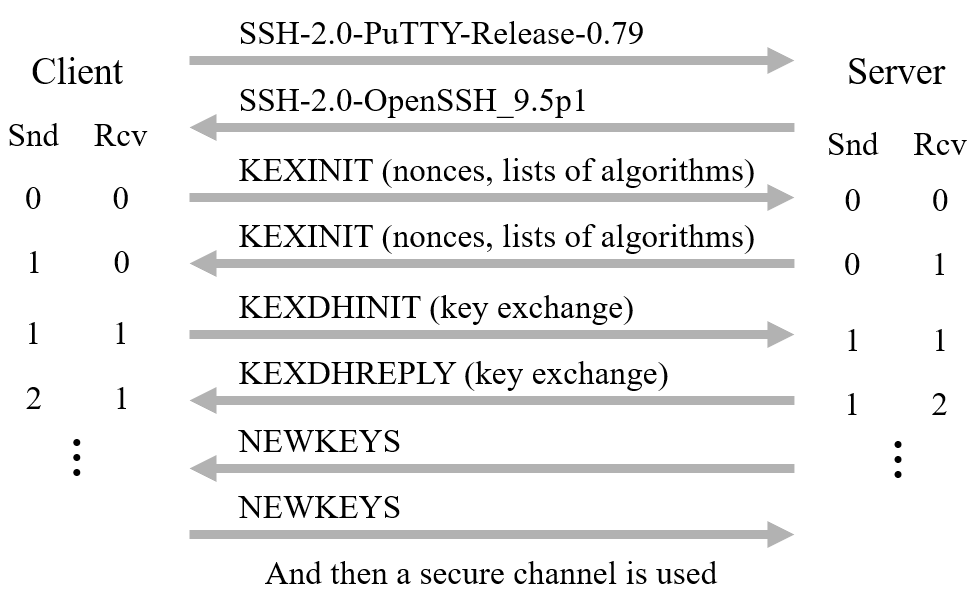
\includegraphics[width=0.6\linewidth]{diagrams-i-made/Basic-SSH-handshake.png}
    \caption{Typical SSH Handshake before the secure channel is used. The numbers on the sides count the number of packets sent and received.}
    \label{fig:basic-SSH-handshake}
\end{figure}


\section{SSH handshake}
\label{sec:SSH-handshake}

The handshake is displayed on \autoref{fig:basic-SSH-handshake}. The Binary Packet Protocol (BPP) is used to perform the SSH handshake. Most information on this paper about the SSH handshake and SSH downgrade is from \cite{terrapin-attack}. The main purpose of the handshake is to exchange information to set up the secure channel. In the secure channel, each packet sent is encrypted and with Message Authentication Code (MAC). This MAC is verified by the receiver to make the exchange safer. Here is a description of the following steps of the handshake:

\begin{enumerate}

    \item Both parties start by exchanging their versions.
    
    \item The \textsc{KexInit} messages contain nonces. (In cryptography, a nonce is a random generated number, that make the encrypted message harder to decrypt, because it is less predictable.) Those messages also contain lists of algorithms, e.g. two for the encryption (for both directions), one for the MAC. Which algorithm is actually used depends on the order of both lists. 
    
    \item The \textsc{KexDhInit} and \textsc{KexDhReply} messages are used to perform a finite-field Diffie-Hellman key exchange, or an alternative method to exchange keys.
    
    \item The \textsc{NewKeys} are exchanged.

    \item After that, the packages are sent through the secure channel.
    
\end{enumerate} 

Once in the secure channel, each packet is encrypted and has a MAC. This is a way to add verification of the packets by the client and the server. To prevent a man-in-the-middle to reorder the packets, both client and server count the number of packets received and sent, with the \textsc{Snd} and \textsc{Rvc} counters. The \textsc{Snd} counter is used in the MAC computation. If a man-in-the-middle deletes a packet, a peer will realize that there is an offset in the count and will notify the other peer.

But before the secure channel, no encryption, MAC or authentication is used, and this can be exploited. The section \autoref{sec:extension-downgrade} will talk about vulnerabilities in ChaCha20-Poly1305 and CBC-EtM, different encryption modes.

\section{Prefix truncation attack}
\label{sec:prefix-truncation}

\begin{figure}
    \centering
    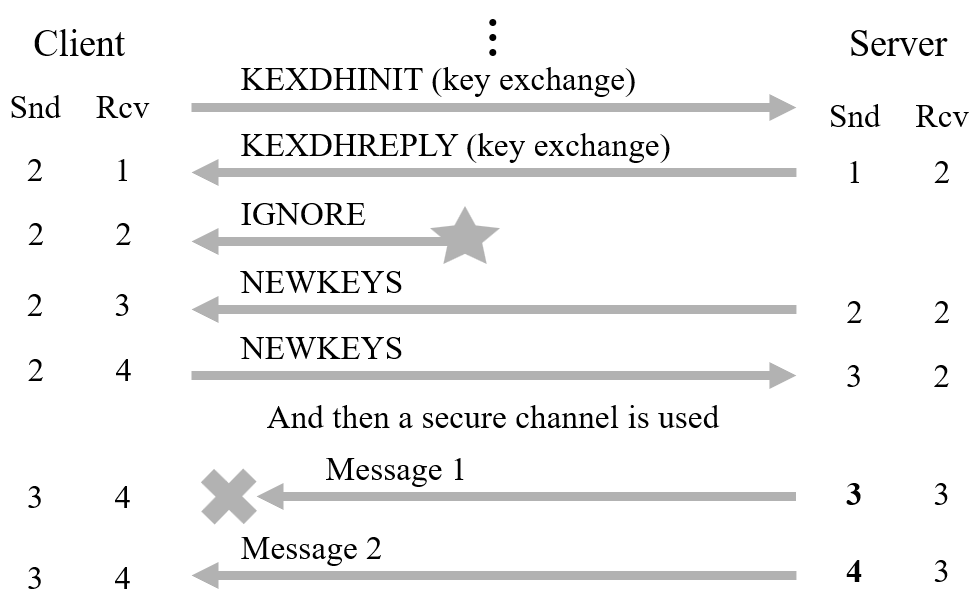
\includegraphics[width=0.6\linewidth]{diagrams-i-made/Basic-prefix-truncation.png}
    \caption{A basic prefix truncation in which a man-in-the-middle sends one \textsc{Ignore} packet to the client during the handshake. The numbers in \textbf{bold} are used for the MAC computation.}
    \label{fig:basic-prefix-truncation}
\end{figure}

A man-in-the-middle can try to offset the counters during the SSH handshake mentioned above in \autoref{sec:SSH-handshake}. Because the secure channel has not started yet, the attacker can simply send raw a message, say the \textsc{Ignore} message, and perform a prefix truncation. In the example given in \autoref{fig:basic-prefix-truncation}, the man-in-the-middle sends the message to the client; once the secure channel is set up, the first packet sent by the server is ignored by the client, because the number \textsc{Snd} decoded from its MAC does not match the client's \textsc{Rcv} counter.

In this example, the purpose of the \textsc{Ignore} message is to protect against traffic analysis, but it is not supposed to have an effect during the handshake.

The way the attack succeeds highly depends on the chosen encryption mode. As soon as the secure channel starts, the way the encryption works will define how likely it is that one of the peers will detect an error. 

\subsection{With ChaCha20-Poly1305}
\label{sec:prefix-truncation-ChaCha20-Poly1305}

ChaCha20 is a stream cipher that encrypts the packet. Then, the Poly1305 authenticator uses the encrypted packet and another key generated by ChaCha20 to create the MAC. This encryption mode only has, as an input, the packet that needs to be decrypted and the sequence number (\textsc{Rcv} or \textsc{Snd}). \cite{ChaCha20-Poly1305-for-IETF-Protocols} \cite{terrapin-attack} This means that the deletion of the first packet \textsc{ExtInfo} will not influence the way the other packets will be decoded. Therefore, truncation attacks are perfectly exploitable for this encryption mode.


\subsection{With CBC-EaM}
\label{sec:prefix-truncation-CBC-EaM}

In this encryption mode, the whole packet is encrypted with CBC (Cypher Block Chaining) and the MAC is generated with EaM (Encrypt and MAC). This means that in order to generate the MAC, EaM uses the unencrypted packet length, the packet encryption and the sequence number (\textsc{Rcv} or \textsc{Snd}). The main problem is that, because of the CBC encryption, each packet is chained, so deleting one alters the decryption of every following packet. With EaM, the MAC verification of a corrupted packet fails very often, preventing the attacker from reaching their goeals.

\subsection{With CBC-EtM}
\label{sec:prefix-truncation-CBC-EtM}

Here, the payload is still encrypted with CBC (Cypher Block Chaining) but the MAC is generated with EtM (Encrypt then MAC). So, in order to generate the MAC, EtM use the sequence number, the unencrypted packet length and the encrypted packet.

This encryption mode has the same effect as CBC-EaM, but this time the corrupted messages result in an error much less often. The way the packet is analyzed by the receiver can give results such as:

\begin{itemize}
    \item The packet is too corrupted and the connection is closed.
    \item The packet has the right padding, but the ID of the message is not recognized, so an \textsc{Unimplemented} response is sent. Using the same notation as in \cite{terrapin-attack}, we will call this type of corruption \textit{Evasively Corrupt}.
\end{itemize}

The likelihood of each result very much depends on the implementation.

If the attacker wants to delete \textit{N} packets, they can choose to delete \textit{N} - 1 packets using the technique of offsetting the sequence number already mentioned in the beginning of this section. There is a chance (depending, again, on the implementation) that the \textit{N}-th packet will be \textit{Evasively Corrupt}, and therefore ignored by the receiver. In this case, the attack is successful.

\section{Extension downgrade attack on OpenSSH 9.4p1 and 9.5p1}
\label{sec:extension-downgrade}

The extension downgrade attack consists of applying a prefix truncation to remove the \textsc{ExtInfo} message that is sent in the secure channel. This will disable most extensions, including:

\begin{itemize}
    \item \textbf{Keystroke timing countermeasures}: In SSH interactive mode, every keystroke that a user types is sent to the remote machine immediately after the key is pressed, which leaks the inter-keystroke timing information of user’s typing. Without the keystroke timing countermeasures, this makes side-channel attacks possible. \cite{keystore-timing-attack}
    \item Disabling the \textbf{server-sig-algs} extension can lead to worse authentication requests. When this is extension enabled, the authentication is done through a public key algorithm. Otherwise, the client will try to authenticate through trial and error, which makes the communication more vulnerable to the attacker. \cite{extension-server-sig-algs}
\end{itemize}

This first \textsc{ExtInfo} package contains information to initiate an extension negotiation between the peers. Other \textsc{ExtInfo} messages can be sent but, in these versions, those ones can not start the negotiation process again.

\subsection{With ChaCha20-Poly1305}
\label{sec:downgrade-ChaCha20-Poly1305}

This attack works well with this encryption mode (for reasons explained in \autoref{sec:prefix-truncation-ChaCha20-Poly1305}), so we simply have to perform the attack shown in \autoref{sec:prefix-truncation} and \autoref{fig:basic-prefix-truncation}. In this attack, the first message of the secure channel is \textsc{ExtInfo}.

\subsection{With CBC-EtM}
\label{sec:downgrade-CBC-EtM}

\begin{figure}
    \centering
    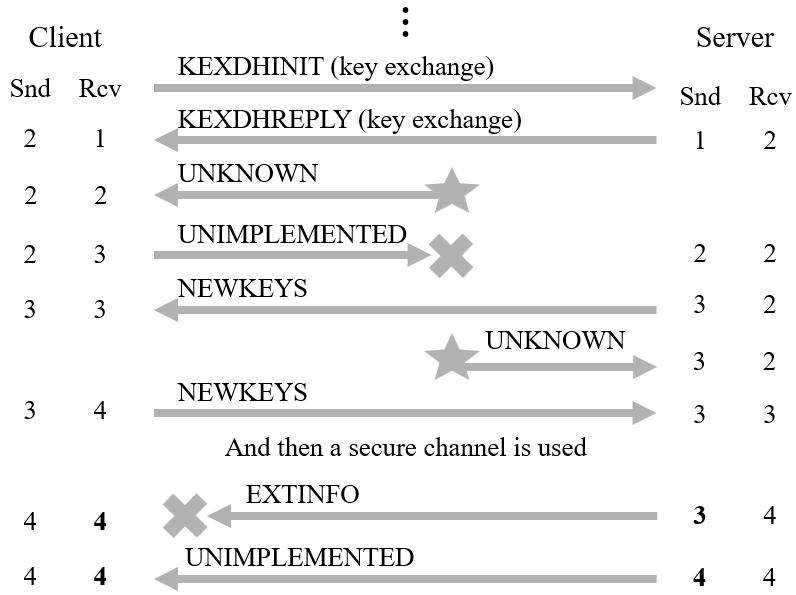
\includegraphics[width=0.55\linewidth]{diagrams-i-made/Extension-downgrade-CBC-EtM.png}
    \caption{Extension downgrade attack on OpenSSH 9.4p1 or 9.5p1, with the encryption mode CBC-EtM}
    \label{fig:extension-downgrade-CBC-EtM}
\end{figure}

The attack with this encryption mode is presented in \autoref{fig:extension-downgrade-CBC-EtM}. In that situation, the aim is to infect the \textsc{ExtInfo} so that it becomes \textit{Evasively Corrupt}, as described in \autoref{sec:prefix-truncation-CBC-EtM}. To offset the count, during the handshake, an unknown message is sent to the client, and its \textsc{Unimplemented} response deleted by the attacker. This way, the MAC verification of the \textsc{ExtInfo} fails. Another unknown packet is sent to the server, but this time, the \textsc{Unimplemented} response is sent in the secure channel. The attacker hopes that this response is only \textit{Evasively Corrupt}, so that the neither peer notices anything. The success rate is low, only around to 3\%.

One way to improve the success rate is by replacing the unknown message sent to the server with a \textsc{Ping} message, which will have its answer \textsc{Pong} sent in the secure channel. Because this message is smaller, the likelihood that it's \textit{Evasively Corrupt} increases to approximately 80\%.


\begin{figure}
    \begin{subfigure}{.48\textwidth}
        \centering
        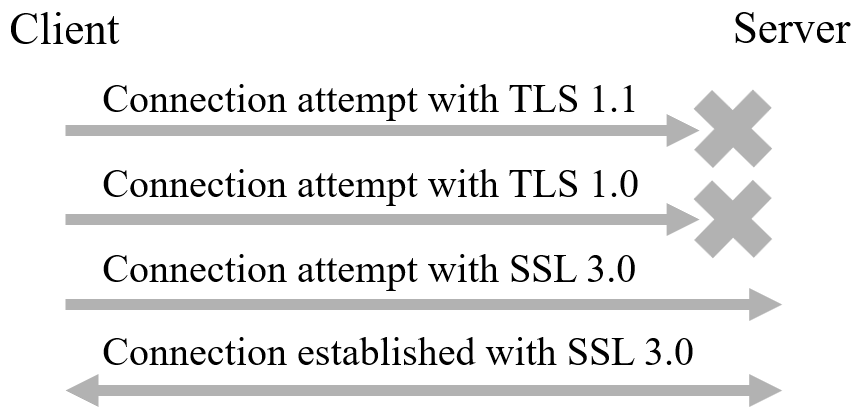
\includegraphics[width=0.9\linewidth]{diagrams-i-made/TLS-dowgrade-attack.png}
        \caption{Basic TLS downgrade attack, where the connection attempts are deleted by a man-in-the-middle.}
        \label{fig:basic-TLS-downgrade-attack}
    \end{subfigure}
    \hfill
    \begin{subfigure}{.48\textwidth}
        \centering
        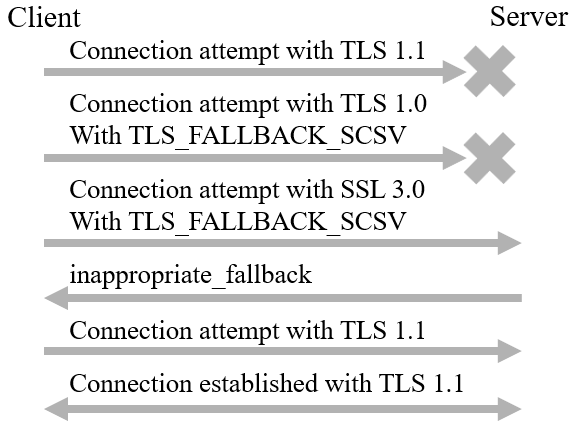
\includegraphics[width=0.9\linewidth]{diagrams-i-made/TLS-dowgrade-protection.png}
        \caption{Schema of how TLS\_FALLBACK\_SCSV helps prevent a downgrade attack. The server here recognizes the FALLBACK SCSV message. Here, the server supports a better version, so it returns the inappropriate\_fallback message.}
        \label{fig:basic-TLS-downgrade-protection}
    \end{subfigure}
    \caption{Schemas about TLS downgrade attacks.}
\end{figure}


\section{TLS downgrade attack}
\label{sec:TLS-downgrade-attack}

A basic TLS downgrade attack is shown in \autoref{fig:basic-TLS-downgrade-attack}. The client attempts to connect to a server, but the connection fails because of the man-in-the-middle (in other cases, the connection can also fail because of a network error). In older procedures, the client would try to connect with older protocols, like older TLS versions and the older SSL versions. That means that the man-in-the-middle, just by intercepting certain packets, could trigger a version downgrade \cite{tls-downgrade-1}.

This downgrade attack is made possible only if TLS\_FALLBACK\_SCSV is not sent by the client \cite{TLS-Fallback-Signaling-Cipher-Suite-Value}. More information about this message can be found in section \autoref{sec:TLS-downgrade-protection}.


\subsection{Downgraded to SSL 3.0}

When the communication is downgraded to SSL 3.0, and if the CBC mode is enabled, the communication becomes vulnerable to a POODLE attack (Padding Oracle On Downgraded Legacy Encryption). This is made possible because the way the encryption functions makes it vulnerable.

Similarly to the way CBC-EtM or CBC-EaM works for SSH (explained in \autoref{sec:prefix-truncation-CBC-EaM} and \autoref{sec:prefix-truncation-CBC-EtM}), a MAC is generated during encryption, and the padding is checked during the decryption. But in the algorithms of these subsections, the minimum size of the padding is 4 \cite{terrapin-attack}, while in SSL 3.0, the padding can be between the cipher's block length and zero \cite{ssl-protocol-ver-3}.

In this context, the oracle can be the server or the client. The way the implementation of SSL reacts to a given block gives the attacker information about if the padding is valid or not. To start the padding oracle attack, the attacker asks the oracle to find a ciphertext with the smallest. Because the padding is put at the end of the block, the information that one ciphertext has valid padding helps us determine the last byte. With this information, we can try to evaluate the second to last byte, and repeat. This attack doesn't need the initialization vector to work.

With a minimum padding of 4, the likelihood that the oracle marks the cipher as valid is close to one out of $255^{4}$. In our case, the padding can be one or zero, so the attack is much more likely to succeed.


\section{TLS downgrade protection}
\label{sec:TLS-downgrade-protection}

This specific downgrade protection is displayed in \autoref{fig:basic-TLS-downgrade-protection}. To avoid downgrade attacks, and on the version TLS 1.0, 1.1 and 1.2, the client sends the TLS\_FALLBACK\_SCSV message each time it attempts a connection with a downgraded version \cite{TLS-Fallback-Signaling-Cipher-Suite-Value}. A man-in-the-middle can not only remove this message from the packet because the handshake is cryptographically protected. But it still mostly does not break backward compatibility, because older TLS and SSL versions just ignore the message.

When a server receives a connection attempt with the TLS\_FALLBACK\_SCSV message, it checks its supported versions. If a better connection is possible, the server returns the inappropriate\_fallback message. The client then restarts connections with better versions. \cite{TLS-Fallback-Signaling-Cipher-Suite-Value}

TLS 1.3 uses a similar mechanism, where the value DOWNGRD01 or DOWNGRD00 must be sent to older TLS or SSL versions. \cite{TLS-1.3-in-Practice}


\bibliographystyle{alpha}
\bibliography{biblio}

\end{document}